\section{Classical density functional theory}
\label{sec:dft}

Classical density functional theory is a general framework for describing inhomogeneous systems.
Although our primary focus will be the homogeneous liquid, many useful results can be obtained from an inhomogeneous description.
We will work primarily from the classic texts Refs.\ \cite{EvansAP1979,Evans1989,EvansFoIF1992}, although we found Refs.\ \cite{AshcroftAJP1996,Hansen2013} to be helpful supplementary texts.

Our intention in this section is to provide more exposition on the various correlation functions which are important for liquid state physics, as well as historical context for the \emph{morphometric approach} which will be the focus of chapters \ref{chapter:morphometric-framework}, \ref{chapter:morphometric-applications} and \ref{chapter:resummation}.
For the latter goal we will introduce its historical antecedent, fundamental measure theory, in section \ref{sec:fmt}.
The morphometric approach will be fully described in subsequent chapters, so we will introduce it here only to provide further context.

\subsection{Inhomogeneous generalisations of the thermodynamic potentials}
\label{sec:inhomogeneous-potentials}

In this section we introduce the inhomogeneous generalisations of the thermodynamic potentials introduced in section \ref{sec:stat-mech}.
These generalisations will provide a route to a fully inhomogeneous theory of fluids, with many useful applications to correlations within the homogeneous fluid.

For inhomogeneous systems the Legendre transform of $\Omega$ \eqref{eq:grand-potential-legendre-transform} generalises to
\begin{equation}
  \Omega = F - \int \rho^{(1)}(\vec{r}) \mu \, d\vec{r}.
\end{equation}
Subtracting external potential contributions from the Helmholtz free energy defines an \emph{intrinsic free energy} containing contributions arising solely from the internal interactions, i.e.\
\begin{equation}\label{eq:intrinsic-free-energy}
  \mathcal{F}
  =
  F - \int \rho^{(1)}(\vec{r}) \phi_\mathrm{ext}(\vec{r}) \, d\vec{r}
\end{equation}
so that the grand potential becomes
\begin{equation}\label{eq:dft-grand-potential}
  \begin{split}
    \Omega
    &=
    \mathcal{F}
    - \int \rho^{(1)}(\vec{r}) (\mu - \phi_\mathrm{ext}(\vec{r})) \, d\vec{r}
    \\ &=
    \mathcal{F}
    - \int \rho^{(1)}(\vec{r}) \psi(\vec{r}) \, d\vec{r}
  \end{split}
\end{equation}
where we defined the \emph{intrinsic chemical potential} $\psi(\vec{r}) = \mu - \phi_\mathrm{ext}(\vec{r})$ in the final step.

Furthermore, the intrinsic free energy can be decomposed into an \emph{ideal} and \emph{excess} part as in
\begin{equation}\label{eq:F-decomposition}
  \mathcal{F}
  =
  \mathcal{F}^\mathrm{id} +
  \mathcal{F}^\mathrm{ex}.
\end{equation}
The excess component emerges as from the interactions between particles and in general it is intractably hard to determine this exactly except in special limits (e.g.\ in the one-dimensional limit).
As such, approximate forms for $\mathcal{F}^\mathrm{ex}$ must be used in general which contrains the success of applications of DFT to the accuracy of this contribution.
By contrast, the ideal component can be computed explicitly.
The partition function for the ideal gas is easily calculated giving
\begin{equation}\label{eq:ideal-grand-canonical-partition}
  \Xi^\mathrm{id}
  =
  \sum_{N=0}^\infty
  \frac{(e^{\beta\mu} Z_1)^N}{N!}
  =
  \exp{\left( \frac{Z_1 e^{\beta \mu}}{\Lambda^d} \right)}.
\end{equation}
Then, following Ref.\ \cite{AshcroftAJP1996}, we write the equilibrium single-particle density as
\begin{equation*}
  \rho^{(1)}(\vec{r})
  =
  \left\langle
  \sum_{i=1}^N \delta(\vec{r} - \vec{r}_i)
  e^{-\beta \phi_\mathrm{ext}(\vec{r})}
  \right\rangle
\end{equation*}
which in the absence of particle interactions reduces to
\begin{equation}\label{eq:ideal-density}
  \rho^{(1)}(\vec{r})
  =
  \frac{
    \langle N \rangle e^{-\beta \phi_\mathrm{ext}(\vec{r})}
  }{
    \int e^{-\beta \phi_\mathrm{ext}(\vec{r}')} \, d\vec{r}'
  }
  =
  \frac{e^{-\beta (\mu - \phi_\mathrm{ext}(\vec{r}))}}{\Lambda^d}.
\end{equation}
We can express the grand potential for the non-interacting system as a functional of the external potential from the partition function \eqref{eq:ideal-grand-canonical-partition} as
\begin{equation*}
  \beta\Omega^\mathrm{id}
  =
  - \ln{\Xi^\mathrm{id}}
  =
  - \int \frac{e^{-\beta (\phi_\mathrm{ext}(\vec{r}) - \mu)}}{\Lambda^d} d\vec{r}
\end{equation*}
or in its dual form as a functional of density \eqref{eq:dft-grand-potential} as
\begin{equation*}
  \beta\Omega^\mathrm{id}
  =
  \beta \mathcal{F}^\mathrm{id}
  - \int \rho^{(1)}(\vec{r}) \beta \psi(\vec{r}) \, d\vec{r}.
\end{equation*}
Equating these two forms and rearranging we find the ideal part of the Helmholtz free energy as
\begin{align}
  \beta \mathcal{F}^\mathrm{id}
  &=
  \int
  \left(
  \rho^{(1)}(\vec{r}) \beta (\phi_\mathrm{ext}(\vec{r}) - \mu)
  - \frac{e^{-\beta (\phi_\mathrm{ext}(\vec{r}) - \mu)}}{\Lambda^d}
  \right)
  d\vec{r}
  \nonumber \\ &=
  \int
  \rho^{(1)}(\vec{r})
  \left(
  \ln{(\Lambda^d \rho^{(1)}(\vec{r}))} - 1
  \right)
  d\vec{r}
  \label{eq:ideal-free-energy-functional}
\end{align}
using the ideal density \eqref{eq:ideal-density} in the final step.
The inhomogeneous ideal gas free energy density is thus identical to the homogeneous case \eqref{eq:ideal-free-energy-density} after replacing the global density with a local one.

Armed with functional generalisations of the thermodynamic potentials we can begin to describe the inhomogeneous liquid.
Our focus will be on correlations within the equilibrium liquid, so in the next section we will directly connect the thermodynamic functionals to the correlations functions.

\subsection{Thermodynamic potentials as generating functionals}

Having defined thermodynamic potentials for an inhomogeneous system as functionals, we can make a connection to liquid structure through the various correlation functions.
In sections \ref{sec:liquid-structure} and \ref{sec:virial-series} we saw how the homogeneous correlation functions could obtained from various generating functions.
In the inhomogeneous liquid correlation functions are obtained in a similar way from \emph{generating functionals}.

The fundamental thermodynamic relation describing an infinitesimal change in the Helmholtz free energy, i.e.\
\begin{equation*}
  dF = -S dT - p dV + \mu dN,
\end{equation*}
generalises to an inhomogeneous system as
\begin{equation*}
  \begin{split}
    \delta F
    =
    - S \delta T
    + \int \rho^{(1)}(\vec{r}) \delta \phi_\mathrm{ext}(\vec{r}) \, d\vec{r}
    + \int \mu \delta \rho^{(1)}(\vec{r}) \, d\vec{r}
  \end{split}
\end{equation*}
The change in the intrinsic free energy is then
\begin{equation}\label{eq:infinitesimal-free-energy}
  \begin{split}
    \delta \mathcal{F}
    &=
    \delta F
    - \int \delta \rho^{(1)}(\vec{r}) \phi_\mathrm{ext}(\vec{r}) \, d\vec{r}
    - \int \rho^{(1)}(\vec{r}) \delta \phi_\mathrm{ext}(\vec{r}) \, d\vec{r}
    \\ &=
    - S \delta T
    + \int \delta \rho^{(1)}(\vec{r}) \psi(\vec{r}) \, d\vec{r}.
  \end{split}
\end{equation}
By similar steps, or using the Legendre transform of the grand potential \eqref{eq:grand-potential-legendre-transform}, it follows that
\begin{equation}\label{eq:infinitesimal-grand-potential}
  \delta \Omega
  =
  - S \delta T
  - \int \rho^{(1)}(\vec{r}) \delta \psi(\vec{r}) \, d\vec{r}
\end{equation}
Hence, from functional differentiation of \eqref{eq:infinitesimal-free-energy} and \eqref{eq:infinitesimal-grand-potential} it follows that
\begin{align}
  \label{eq:psi-generator}
  \frac{\delta \mathcal{F}}{\delta \rho^{(1)}(\vec{r})}
  &=
  \psi(\vec{r}),
  \\
  \label{eq:rho-generator}
  \frac{\delta \Omega}{\delta \psi(\vec{r})}
  &=
  - \rho^{(1)}(\vec{r}),
\end{align}
i.e.\ the intrinsic free energy and grand potentials act as \emph{generating functionals} for the intrinsic chemical potential and density respectively.

Repeated functional differentiation of the thermodynamic potentials produces a whole hierarchy of correlation functions.
The hierarchy obtained from the grand potential gives the density-density correlations which we already introduced in \eqref{eq:density-density-correlations};
these are generated by the grand potential as \cite{Hansen2013}
\begin{equation}\label{eq:density-density-generator}
  H^{(n)}(\vec{r}^n)
  =
  - \frac{
    \delta^n \beta \Omega
  }{
    \delta \beta\psi(\vec{r}_1) \cdots \delta \beta\psi(\vec{r}_n)
  }
  =
  \frac{
    \delta^{n-1} \rho^{(1)}(\vec{r}_1)
  }{
    \delta \beta\psi(\vec{r}_2) \cdots \delta \beta\psi(\vec{r}_n)
  }.
\end{equation}
The intrinsic free energy also generates a new hierarchy of correlation functions, however the contribution from the ideal part is not especially interesting.
We thus define the \emph{direct correlation functions} as the hierarchy generated from the excess part as
\begin{equation}\label{eq:direct-correlations}
  c^{(n)}(\vec{r}^n)
  =
  - \frac{
    \delta^n \beta \mathcal{F}^\mathrm{ex}
  }{
    \delta \rho^{(1)}(\vec{r}_1) \cdots \delta \rho^{(1)}(\vec{r}_n)
  }.
\end{equation}
These correlation functions form the basis of integral equation theories which we will outline in the next section.

\subsection{Equilibrium conditions}
\label{sec:oz-equation}

In the preceding sections we defined the thermodynamic potentials for an inhomogeneous system in equilibrium with density profile $\rho(\vec{r}) = \rho^{(1)}(\vec{r})$.
However, we can imagine the generalisation where the equilibrium profile $\rho^{(1)}(\vec{r})$ is replaced by an arbitrary $\rho(\vec{r})$ so
\begin{align*}
  \Omega &\to \Omega[\rho(\vec{r})],
  \\
  \mathcal{F}^\mathrm{id} &\to \mathcal{F}^\mathrm{id}[\rho(\vec{r})],
  \\
  \mathcal{F}^\mathrm{ex} &\to \mathcal{F}^\mathrm{ex}[\rho(\vec{r})].
\end{align*}
These generalised functionals are not strictly the same as the thermodynamic potentials, which only concern equilibrium properties, but there is an important correspondence between them.
Focusing on the grand potential, the following two properties are provable%
\marginfootnote{Full accounts of the classical arguments can be found in Refs.\ \cite{MerminPR1965,EvansAP1979}, and a more compact argument has recently been formulated in Ref.\ \cite{DwandaruPRE2011}.}:
\begin{enumerate}
  \item It is bounded from below by the grand potential, i.e.\
    \begin{equation*}
      \Omega[\rho(\vec{r})] \ge \Omega.
    \end{equation*}
  \item Equality with the grand potential occurs \emph{only} in the case of the equilibrium density profile, i.e.\
    \begin{equation*}
      \Omega[\rho^{(1)}(\vec{r})] = \Omega.
    \end{equation*}
\end{enumerate}
These two properties can be elegantly summarised by the \emph{variational principle}
\begin{equation}\label{eq:dft-equilibrium}
  \left.
  \frac{\delta \Omega}{\delta \rho^{(1)}(\vec{r})}
  \right|_{\rho(\vec{r}) = \rho^{(1)}(\vec{r})}
  =
  0,
\end{equation}
which provides the route to numerical applications of DFT; minimisation of the grand potential with respect to density is sufficient to determine the equilibrium density profile and its corresponding free energy.

To bring the variational principle to more practical use we can insert the functional form of the grand potential deduced in section \ref{sec:inhomogeneous-potentials} into \eqref{eq:dft-equilibrium} giving
\begin{equation*}
  %\frac{\delta \Omega}{\delta \rho^{(1)}(\vec{r})}
  %= 0
  %% &=
  %% \frac{\delta \mathcal{F}}{\delta \rho^{(1)}(\vec{r})}
  %% - \frac{\delta}{\delta \rho(\vec{r}')}
  %% \left(
  %% \int \rho(\vec{r}) \psi(\vec{r})
  %% \, d\vec{r}
  %% \right)
  %\\ &=
  %  =
  \frac{\delta \mathcal{F}}{\delta \rho^{(1)}(\vec{r})}
  - \psi(\vec{r})
  =
  \int
  \rho^{(1)}(\vec{r}') \frac{\delta \psi(\vec{r})'}{\delta \rho^{(1)}(\vec{r})}
  \, d\vec{r}'.
\end{equation*}
The separate condition \eqref{eq:psi-generator} causes the first two terms to cancel, leading to the two equilibrium conditions
\begin{subequations}
  \begin{align}
    \label{eq:fmt-psi-equilibrium}
    \frac{\delta \mathcal{F}^\mathrm{id}[\rho(\vec{r})]}{\delta \rho(\vec{r}')}
    + \frac{\delta \mathcal{F}^\mathrm{ex}[\rho(\vec{r})]}{\delta \rho(\vec{r}')}
    &=
    \psi(\vec{r}),
    \\
    \int
    \rho^{(1)}(\vec{r}) \frac{\delta \psi(\vec{r})}{\delta \rho^{(1)}(\vec{r}')}
    \, d\vec{r}
    &=
    0,
  \end{align}
\end{subequations}
of which the first is most useful.
The first functional derivative of the ideal intrinsic free energy \eqref{eq:ideal-free-energy-functional} yields
\begin{equation*}
  \frac{
    \delta \beta \mathcal{F}^\mathrm{id}
  }{
    \delta \rho^{(1)}(\vec{r})
  }
  =
  \ln{(\Lambda^d \rho^{(1)}(\vec{r}))},
\end{equation*}
and with the excess term is the generating functional of $c^{(n)}$ \eqref{eq:direct-correlations} we obtain
\begin{equation*}
  \ln{(\Lambda^d \rho^{(1)}(\vec{r}))}
  - c^{(1)}(\vec{r})
  =
  \psi(\vec{r})
\end{equation*}
or rearranged for the density
\begin{equation}\label{eq:equilibrium-density}
  \rho^{(1)}(\vec{r})
  =
  \frac{
    \exp{\left(\beta\psi(\vec{r}) + c^{(1)}(\vec{r})\right)}
  }{ \Lambda^d }.
\end{equation}
This equation provides the basis for iterative schemes to solve \eqref{eq:dft-equilibrium} (see e.g.\ \cite{RothJPCM2010}).
Importantly, this process incorporates an arbitrary external potential inside $\psi(\vec{r})$ which could represent e.g.\ a test-particle inserted into the liquid so that the grand potential represents a chemical potential.
This example provides a potential way of using an inhomogeneous framework to approach the homogeneous liquid, illustrating the usefulness of the DFT formalism.

Further functional derivatives of the equilibrium condition provides a whole hierarchy of equivalent equilibrium criteria.
Of particular note is the next equation in the hierarchy, the Ornstein-Zernike equation, which forms the basis of integral theories of the liquid state%
\marginfootnote{Conventionally this class of theories is presented in its own right rather than as a special case of density functional theory; we opted for this more modern presentation to be marginally more economical with chapter length.}.
This connects the density-density and direct correlation functions through the chain rule of functional calculus, i.e.\
\begin{equation}\label{eq:oz-chain-rule}
  \delta(\vec{r}_1 - \vec{r}_2) =
  \int
  \frac{\delta \rho^{(1)}(\vec{r}_1)}{\delta \beta\psi(\vec{r}')}
  \frac{\delta \beta\psi(\vec{r}')}{\delta \rho^{(1)}(\vec{r}_2)}
  \, d\vec{r}'.
\end{equation}
The first term appearing in the integrand is simply the pair density-density correlation function $H^{(2)}$ via \eqref{eq:density-density-generator},
so we will require an explicit expression for the second term to proceed.

We require the functional derivative of $\psi(\vec{r})$ corresponding to the second functional derivatives of the intrinsic free energy through \eqref{eq:fmt-psi-equilibrium}.
To obtain the higher order functional derivatives of the ideal term, it is helpful to write it as an integral with a delta function
\begin{equation*}
  \frac{
    \delta \beta \mathcal{F}^\mathrm{id}
  }{
    \delta \rho^{(1)}(\vec{r})
  }
  =
  \int \delta{(\vec{r}' - \vec{r})}
  \ln{(\Lambda^d \rho^{(1)}(\vec{r}'))} \, d\vec{r}',
\end{equation*}
so we can obtain the second derivative as
\begin{equation*}
  \frac{
    \delta^2 \beta \mathcal{F}^\mathrm{id}
  }{
    \delta \rho^{(1)}(\vec{r}) \delta \rho^{(1)}(\vec{r}')
  }
  =
  \frac{\delta(\vec{r}'-\vec{r})}{\rho^{(1)}(\vec{r})}.
\end{equation*}
%% Iterating this procedure gives us the $n$th functional derivative as
%% \begin{equation}
%%   \begin{split}
%%     \frac{
%%       \delta^n \beta \mathcal{F}^\mathrm{id}
%%     }{
%%       \delta \rho^{(1)}(\vec{r}_1) \cdots \delta \rho^{(1)}(\vec{r}_n)
%%     }
%%     &=
%%     \frac{
%%       \partial^{n-1} (\ln{(\Lambda^d \rho^{(1)}(\vec{r}))})
%%     }{
%%       \partial \rho^{(1)}(\vec{r})^{n-1}
%%     }
%%     \prod_{i=2}^n \delta(\vec{r}_i - \vec{r}_1)
%%     \\ &=
%%     (-1)^{n-1}
%%     \frac{(n-2)!}{\rho^{(1)}(\vec{r})^{n-1}}
%%     \prod_{i=2}^n \delta(\vec{r}_i - \vec{r}_1),
%%   \end{split}
%% \end{equation}
%% where the last line is valid for all $n \ge 2$.
Functional differentiation of \eqref{eq:fmt-psi-equilibrium} then yields
\begin{equation*}\label{eq:intrinsic-chemical-potential-inverse-derivative}
  \frac{\delta \beta \psi(\vec{r})}{\delta \rho^{(1)}(\vec{r}')}
  =
  \frac{\delta(\vec{r} - \vec{r}')}{\rho^{(1)}(\vec{r}')}
  - c^{(2)}(\vec{r}, \vec{r}').
\end{equation*}
using the definition of the direct correlation function \eqref{eq:direct-correlations} in the latter step.
Inserting this expression into \eqref{eq:oz-chain-rule} gives
\begin{equation*}
  \begin{split}
    \delta(\vec{r}_1 - \vec{r}_2)
    &=
    \int
    H^{(2)}(\vec{r}_1, \vec{r}')
    \left(
    \frac{\delta(\vec{r}' - \vec{r}_2)}{\rho^{(1)}(\vec{r}')} -
    c^{(2)}(\vec{r}', \vec{r}_2)
    \right)
    \, d\vec{r}'
    %% \\ &=
    %% \rho^{(1)}(\vec{r}_1)
    %% \left(
    %% h^{(2)}(\vec{r}_1, \vec{r}_2) -
    %% c^{(2)}(\vec{r}_1, \vec{r}_2)
    %% \right) +
    %% \delta(\vec{r}_1 - \vec{r}_2) -
    %% \\ &\qquad
    %% \rho^{(1)}(\vec{r}_1)
    %% \int
    %% \rho^{(1)}(\vec{r}')
    %% h^{(2)}(\vec{r}_1, \vec{r}')
    %% c^{(2)}(\vec{r}', \vec{r}_2)
    %% \, d\vec{r}'
  \end{split}
\end{equation*}
which upon inserting the definition of $H^{(2)}$ from \eqref{eq:pair-density-density-correlation} rearranges to give the Ornstein-Zernike equation
\begin{equation}\label{eq:ornstein-zernike-generic}
  h^{(2)}(\vec{r}_1, \vec{r}_2) =
  c^{(2)}(\vec{r}_1, \vec{r}_2) +
  \int
  \rho^{(1)}(\vec{r}')
  h^{(2)}(\vec{r}_1, \vec{r}')
  c^{(2)}(\vec{r}', \vec{r}_2)
  \, d\vec{r}',
\end{equation}
which is a classic result of liquid state theory (cf.\ Refs.\ \cite{OrnsteinPAS1914,Hansen2013,EvansAP1979}).

\begin{tcolorbox}[title=Ornstein-Zernike equation for a uniform simple liquid]
For a uniform liquid interacting through a spherically symmetric pair potential the Ornstein-Zernike equation becomes
\begin{equation}\label{eq:ornstein-zernike-spherical}
  \begin{split}
    h^{(2)}(r)
    &=
    c^{(2)}(r) +
    \rho
    \int
    h^{(2)}(r)
    c^{(2)}(|\vec{r}' - \vec{r}|)
    \, d\vec{r}'
    \\ &=
    c^{(2)}(r) + \rho \, (h^{(2)} * c^{(2)})(r),
  \end{split}
\end{equation}
where $r = |\vec{r}_2 - \vec{r}_1|$ and $(f*g)(\vec{r})$ denotes a convolution between functions $f$ and $g$.
In Fourier space the convolution becomes a product so we obtain
\begin{equation*}
  \tilde{h}^{(2)}(\vec{k})
  =
  \tilde{c}^{(2)}(\vec{k}) +
  \rho \, \tilde{h}^{(2)}(\vec{k}) \tilde{c}^{(2)}(\vec{k})
\end{equation*}
where the tildes over a function denotes its Fourier transform.
This rearranges to give
\begin{equation*}
  \tilde{h}^{(2)}(\vec{k})
  =
  \frac{\tilde{c}^{(2)}(\vec{k})}{1 - \rho \tilde{c}^{(2)}(\vec{k})}
\end{equation*}
which gives the static structure factor \eqref{eq:static-structure-factor} as
\begin{equation*}
  S^{(2)}(\vec{k})
  =
  \rho \delta(\vec{k}) +
  \frac{1}{1 - \rho \tilde{c}^{(2)}(\vec{k})}.
\end{equation*}
\end{tcolorbox}

If the pair direct correlation function is known it is thus straightforward to obtain the equation of state through the compressibility route \eqref{eq:compressibility-route-pressure}
\begin{equation*}
  \frac{\beta p}{\rho}
  =
  1 - \frac{1}{\rho} \int_0^\rho \tilde{c}^{(2)}(0) \rho' d\rho'.
\end{equation*}
The main task in an integral equation approach is to find an approximate closure for $c^{(2)}$ in order to solve the Ornstein-Zernike equation.
The process of determining the direct correlation functions is equivalent (at least formally) to finding its generating functional $\mathcal{F}^\mathrm{ex}$.

%% \subsection{Generalised Ornstein-Zernike equations}

%% This section follows \cite{BarratMP1988}.\todo{Check this reference and rewrite accordingly}

%% Thus for higher $n$ we have
%% \begin{equation}
%%   \begin{split}
%%     c^{(n)}(\vec{r}^n)
%%     &=
%%     \frac{
%%       \delta^{n-1} c^{(1)}(\vec{r}_1)
%%     }{
%%       \delta \rho^{(1)}(\vec{r}_2) \cdots \delta \rho^{(1)}(\vec{r}_n)
%%     }
%%     \\ &=
%%     (-1)^n
%%     \frac{(n-2)!}{\rho^{(1)}(\vec{r}_1)^{n-1}}
%%     \prod_{i=2}^n \delta(\vec{r}_i - \vec{r}_1)
%%     - \frac{
%%       \delta^{n-1} \beta\psi(\vec{r}_1)
%%     }{
%%       \delta \rho^{(1)}(\vec{r}_2) \cdots \delta \rho^{(1)}(\vec{r}_n)
%%     }
%%   \end{split}
%% \end{equation}
%% or
%% \begin{equation}
%%   \frac{\delta^{n-1} \beta\psi(\vec{r}_1)}{\delta \rho^{(1)}(\vec{r}_2) \cdots \delta \rho^{(1)}(\vec{r}_n)}
%%   =
%%   (-1)^n
%%   \frac{(n-2)!}{\rho^{(1)}(\vec{r}_1)^{n-1}}
%%   \prod_{i=2}^n \delta(\vec{r}_i - \vec{r}_1)
%%   - c^{(n)}(\vec{r}^n)
%% \end{equation}

%% \begin{equation*}
%%   H^{(n)}(\vec{r}^n)
%%   =
%%   \frac{
%%     \delta^{n-1} \rho^{(1)}(\vec{r}_1)
%%   }{
%%     \delta \beta\psi(\vec{r}_2) \cdots \delta \beta\psi(\vec{r}_n)
%%   }.
%% \end{equation*}

%% Defining
%% \begin{equation*}
%%   K^{(n)}(\vec{r}^n)
%%   =
%%   \frac{
%%     \delta^{n-1} \beta\psi(\vec{r}_1)
%%   }{
%%     \delta \rho^{(1)}(\vec{r}_2) \cdots \delta \rho^{(1)}(\vec{r}_n)
%%   }
%% \end{equation*}
%% we have
%% \begin{equation*}
%%   \frac{
%%     \delta K^{(n)}(\vec{r}^n)
%%   }{
%%     \delta \rho^{(1)}(\vec{r}_{n+1})
%%   }
%%   =
%%   K^{(n+1)}(\vec{r}^{n+1}).
%% \end{equation*}
%% and
%% \begin{equation*}
%%   \begin{split}
%%     \frac{\delta H^{(n)}(\vec{r}^n)}{\delta \rho^{(1)}(\vec{r}_{n+1})}
%%     &=
%%     \int
%%     \frac{\delta H^{(n)}(\vec{r}^n)}{\delta \psi(\vec{r}')}
%%     \frac{\delta \psi(\vec{r}')}{\delta \rho^{(1)}(\vec{r}_{n+1})}
%%     \, d\vec{r}' \\
%%     &=
%%     \int
%%     H^{(n+1)}(\vec{r}^n, \vec{r}')
%%     K^{(2)}(\vec{r}', \vec{r}_{n+1})
%%     \, d\vec{r}' \\
%%     &=
%%     H^{(n+1)} * K^{(2)}(\vec{r}^{n+1}).
%%   \end{split}
%% \end{equation*}
%% In this form the Ornstein-Zernike equation can be written.
%% \begin{equation*}
%%   \begin{split}
%%     \delta(\vec{r}_1 - \vec{r}_2)
%%     &=
%%     \int
%%     \frac{\delta \rho^{(1)}(\vec{r}_1)}{\delta \psi(\vec{r}')}
%%     \frac{\delta \psi(\vec{r}')}{\delta \rho^{(1)}(\vec{r}_2)}
%%     \, d\vec{r}' \\
%%     &=
%%     \int
%%     H^{(2)}(\vec{r}_1, \vec{r}') K^{(2)}(\vec{r}', \vec{r}_2)
%%     \, d\vec{r}' \\
%%     &=
%%     H^{(2)} * K^{(2)} (\vec{r}^2)
%%   \end{split}
%% \end{equation*}
%% Taking functional derivatives of this expression gives us a hierarchy of generalised Ornstein-Zernike equations.
%% For example, the next equation in the hierarchy is
%% \begin{equation*}
%%   H^{(2)} * K^{(3)} (\vec{r}^3) +
%%   H^{(3)} * K^{(2)} * K^{(2)} (\vec{r}^3)
%%   = 0
%% \end{equation*}
%% The next functional derivative
%% \begin{equation}
%%   \begin{split}
%%   H^{(2)} * K^{(4)} (\vec{r}^4) & \\
%%   + \; 3 H^{(3)} * K^{(3)} * K^{(2)} (\vec{r}^4) & \\
%%   + \; H^{(4)} * K^{(2)} * K^{(2)} * K^{(2)} (\vec{r}^4)
%%   &= 0
%%   \end{split}
%% \end{equation}
%% And the next one%
%% \todo{Can we find a general formula? I notice some constraints on the indices: the sum of the indices $\{m\}$ in the $K^{(m)}$ terms must add up to $n-1$ so that the right number of independent variables are returned (the extra one is provided by the $H^{(l)}$ function giving the $\vec{r}^n$ total.)}
%% \begin{equation}
%%   \begin{split}
%%     H^{(2)} * K^{(5)} (\vec{r}^5) & \\
%%     + \; 3 H^{(3)} * K^{(3)} * K^{(3)} (\vec{r}^5) & \\
%%     + \; 4 H^{(3)} * K^{(4)} * K^{(2)} (\vec{r}^5) & \\
%%     + \; 6 H^{(4)} * K^{(3)} * K^{(2)} * K^{(2)} (\vec{r}^5) & \\
%%     + \; H^{(5)} * K^{(2)} * K^{(2)} * K^{(2)} * K^{(2)} (\vec{r}^5)
%%     &=
%%     0
%%   \end{split}
%% \end{equation}

\subsection{Fundamental measure theory}
\label{sec:fmt}

DFT provides an elegant framework for treating the inhomogeneous liquid, however as we have shown any application is limited by the accuracy of the (excess) intrinsic free energy.
%Hitherto we have not given any indication over how one might approximate this quantity, which is a hard problem in general.
It is a hard problem in general to derive accurate approximations to $\mathcal{F}^\mathrm{ex}$; however, for hard spheres%
\marginfootnote{We concentrate on hard spheres here, however we note that generalisations exist for hard particle systems of more general shapes \cite{RosenfeldPRE1994,RosenfeldMP1995,Hansen-GoosPRL2009, Hansen-GoosJPCM2010}.
  The more recent works are accurate enough to capture isotropic--nematic transitions in the fluid.
}
it is possible to exploit ideas from integral geometry (section \ref{sec:integral-geometry}) and derive a highly accurate class of free energy functionals.
In this section we describe fundamental measure theory (FMT), which provides the most successful theory for inhomogeneous hard sphere systems.
We mainly follow Refs.\ \cite{RothJPCM2010,SantosPRE2012}, but we mention also the review \cite{LutskoAiCP2010} which has more of a focus on crystallisation.
\todo{Insert reference (foreshadowing) to this section in the earlier integral geometry section.}

To introduce this topic we will first consider the free energy of the homogeneous system, and then generalise to the inhomogeneous one.
Noting that the free energy is determined from the free energy density through
\begin{equation*}
  \beta \mathcal{F}^\mathrm{ex} = \int_V \beta f^\mathrm{ex} \, d\vec{r},
\end{equation*}
we can make a correspondence with the virial series expression for the free energy density \eqref{eq:virial-series-excess-free-energy}.
Using the virial coefficients for an $m$-component mixture \eqref{eq:virial-coefficients-mixtures}, the free energy density in the dilute limit becomes%
\marginfootnote{In this step we are implicitly focusing on systems interacting through pair potentials, where the virial coefficients introduced in section \ref{sec:virial-series} are valid.}
\begin{equation*}
  \beta f^\mathrm{ex}
  =
  - \frac{\rho^2}{2}
  \sum_{i = 1}^m \sum_{j = 1}^m x_i x_j \int_V
  f_{ij}(\vec{r})
  \, d\vec{r}
  + \mathcal{O}(\rho^3).
\end{equation*}
We consider mixtures of hard spheres of radii $R_i$, so The Mayer function $f_{ij}$ must depend on $R_i$ and $R_j$.
%where $\rho_i$ and $R_i$ are the (number) density and radius of species $i$.
The Mayer function for the hard sphere interaction is purely geometric in nature, i.e.\
\begin{equation*}
  -f_{ij}(\vec{r})
  =
  \Theta(R_i + R_j - |\vec{r}|)
\end{equation*}
where $\Theta(\cdot)$ is the Heaviside theta function.
This can be recast in the revealing form
\begin{equation*}\label{eq:hard-mayer-f}
  \begin{split}
    -f_{ij}
    &=
    \begin{cases}
      0 & \textrm{ if } B_i \cap B_j = \emptyset \\
      1 & \textrm{ if } B_i \cap B_j \ne \emptyset
    \end{cases}
    \\ &=
    \chi(B_i \cap B_j)
  \end{split}
\end{equation*}
i.e.\ the Euler characteristic of their intersection.
This allows us to write the free energy density in the dilute limit for a homogeneous system as
\begin{equation*}
  \beta f^\mathrm{ex}
  =
  \frac{\rho^2}{2}
  \sum_{i=1}^m \sum_{j=1}^m
  x_i x_j
  \int_V \chi(B_i \cap B_j(\vec{r})) d\vec{r}
  + \mathcal{O}(\rho^3),
\end{equation*}
or in the notation introduced in section \ref{sec:integral-geometry}
\begin{equation*}
  \beta f^\mathrm{ex}
  =
  \frac{\rho^2}{2}
  \sum_{i=1}^m \sum_{j=1}^m
  x_i x_j
  \int_{G_d} \chi(B_i \cap g B_j) dg
  + \mathcal{O}(\rho^3)
\end{equation*}
which can be evaluated using the principal kinematic formula \eqref{eq:binomial-kinematic-formula}.
Each integral results in $d+1$ terms featuring the intrinsic volumes of the respective particles; we can expect a similar decomposition in the inhomogeneous case.

It is straightforward to generalise the virial series to inhomogeneous systems by localising the the density terms, i.e.\ making the replacement $\rho^n \to \rho(\vec{r}_1) \cdots \rho(\vec{r}_n)$, and bringing them inside the cluster integrals \cite{StillingerJCP1962,RowlinsonPRSA1985}.
The low density free energy then adopts the form
\begin{equation}\label{eq:low-density-inhomogeneous-free-energy}
  \beta \mathcal{F}^\mathrm{ex}[\{\rho_i\}]
  =
  - \frac{1}{2}
  \sum_{i = 1}^m \sum_{j = 1}^m \int_{V^2}
  \rho_i(\vec{r}) \rho_j(\vec{r}')
  f_{ij}(\vec{r} - \vec{r}')
  \, d\vec{r} d\vec{r}'
  + \mathcal{O}(\rho^3).
\end{equation}
Inspired by the intrinsic volumes and the principal kinematic formula, Rosenfeld observed that Mayer function in $d=3$ could be \emph{exactly} decomposed into variants of the intrinsic volumes%
\marginfootnote{Rosenfeld called these \emph{fundamental measures} giving the theory its name.}
\cite{RosenfeldPRL1989}
\begin{equation*}
  \begin{split}
    -f_{ij}(\vec{r})
    =& \quad\,
    \omega_i^{(0)} \otimes \omega_j^{(3)}
    + \omega_i^{(1)} \otimes \omega_j^{(2)}
    + \omega_i^{(2)} \otimes \omega_j^{(1)}
    + \omega_i^{(3)} \otimes \omega_j^{(0)}
    \\ &
    - \omega_i^{(1)} \otimes \omega_j^{(2)}
    - \omega_i^{(2)} \otimes \omega_j^{(1)}
  \end{split}
\end{equation*}
introducing the weight functions
\begin{subequations}
  \begin{align}
    \omega_3^i(\vec{r})
    &=
    \Theta(R_i - r),
    \\
    \omega_2^i(\vec{r})
    &=
    \delta(R_i - r),
    \\
    \omega_1^i(\vec{r})
    &=
    \frac{\omega_2^i(\vec{r})}{4\pi R_i},
    \\
    \omega_0^i(\vec{r})
    &=
    \frac{\omega_2^i(\vec{r})}{4\pi R_i^2},
    \\
    \vec{\omega}_2^i(\vec{r})
    &=
    \frac{\vec{r}}{r} \delta(R_i - r),
    \\
    \vec{\omega}_1^i(\vec{r})
    &=
    \frac{\vec{\omega}_1^i(\vec{r})}{4\pi R_i}.
  \end{align}
\end{subequations}
The appearance of the weight functions inside the free energy \eqref{eq:low-density-inhomogeneous-free-energy} through the Mayer function naturally leads to convolutions with the density.
This gives rise to a set of \emph{weighted densities} defined as \cite{RosenfeldPRL1989,PercusJSP1988}
\begin{equation}
  n_\alpha(\vec{r})
  =
  \sum_{i=1}^m \int_V
  \rho_i(\vec{r}') \, \omega_\alpha^i(\vec{r} - \vec{r'})
  \, d\vec{r}'
\end{equation}
where we use shorthand such that $\alpha$ indexes both the scalar and vector weight functions.
The low density excess free energy becomes a local function of the (nonlocal) weighted densities, as in
\begin{equation*}
  \beta \mathcal{F}^\mathrm{ex}[\{\rho_i\}]
  =
  \int_V \Big(
  n_0(\vec{r}) n_3(\vec{r})
  + n_1(\vec{r}) n_2(\vec{r})
  - \vec{n}_1(\vec{r}) \cdot \vec{n}_2(\vec{r})
  \Big) d\vec{r}
  + \mathcal{O}(\rho^2).
\end{equation*}
Fortuitously, all of the molarity information has been absorbed into the definition of the weighted densities, so the final form contains no explicit mixture dependence; this is an example of a truncatable free energy (section \ref{sec:truncatable-free-energy}).

To generalise the exact dilute limit result to arbitrary densities, we postulate that the free energy remains a functional of density \emph{only} through the weighted densities $\{n_\alpha\}$; this is the central assumption of FMT.

We start by writing the chemical potential of species $i$ as
\begin{equation}\label{eq:fmt-chemical-potential}
  \beta \mu_i^\mathrm{ex}
  =
  \left(
  \frac{\partial \beta f^\mathrm{ex}}{\partial \rho_i}
  \right)_{V,T}.
\end{equation}
In the large particle limit the chemical potential is simply the work required to create a cavity large enough to contain the particle%
\marginfootnote{We will formally derive this property in the context of many-body correlations in section \ref{sec:many-body-correlations}.},
i.e.\ \cite{RothJPCM2002,ReissJCP1960}
\begin{equation}\label{eq:fmt-chemical-potential-pressure}
  \lim_{V_i \to \infty} \frac{\beta \mu_i^\mathrm{ex}}{V_i} = \beta p.
\end{equation}
For concentration dependence which enters only through a finite set of weight functions we have
\begin{equation*}
  \frac{\partial}{\partial \rho_i}
  =
  \sum_\alpha
  \frac{\partial n_\alpha}{\partial \rho_i}
  \frac{\partial}{\partial n_\alpha},
\end{equation*}
of which the explicit differentials give
\begin{subequations}\label{eq:fmt-n-derivatives}
  \begin{align}
    \frac{\partial n_3}{\partial \rho_i}
    &=
    \frac{4 \pi R_i^3}{3},
    \\
    \frac{\partial n_2}{\partial \rho_i}
    &=
    4 \pi R_i^2,
    \\
    \frac{\partial n_1}{\partial \rho_i}
    &=
    R_i,
    \\
    \frac{\partial n_0}{\partial \rho_i}
    &=
    1,
  \end{align}
\end{subequations}
and similar expressions for the vectorial terms.
In the large volume limit the $n_3$ term dominates leading to
\begin{equation*}
  \lim_{V_i \to \infty}
  \frac{\partial}{\partial \rho_i}
  =
  V_i \frac{\partial}{\partial n_3}
\end{equation*}
so it follows from \eqref{eq:fmt-chemical-potential} and \eqref{eq:fmt-chemical-potential-pressure} that
\begin{equation}\label{eq:fmt-pressure}
  \beta p
  =
  \frac{\partial \beta f^\mathrm{ex} }{\partial n_3}.
\end{equation}
Secondly, we find the derivative with respect to density reduces to
\begin{equation*}
  \frac{\partial}{\partial \rho}
  =
  \sum_i
  \frac{\partial \rho_i}{\partial \rho}
  \frac{\partial}{\partial \rho_i}
  =
  \frac{1}{\rho}
  \sum_\alpha
  n_\alpha
  \frac{\partial}{\partial n_\alpha}.
\end{equation*}
Combining these two expressions leads to the scaled particle%
\marginfootnote{We will leave discussion of scaled particle theory until chapter  \ref{chapter:morphometric-framework} where we describe it in detail.}
differential equation \cite{RosenfeldPRL1989}
\begin{equation}\label{eq:fmt-spt-pde}
  (1 - n_3) \frac{\partial f^\mathrm{ex}}{\partial n_3}
  =
  n_0 - f^\mathrm{ex}
  + \sum_{\alpha = 0}^2
  n_\alpha \frac{\partial f^\mathrm{ex}}{\partial n_\alpha}
\end{equation}
In Refs.\ \cite{SantosJCP2012,SantosPRE2012} it was shown that the solution to \eqref{eq:fmt-spt-pde} which correctly recovers the low density behaviour and maximises self-consistency for mixtures must have the generic form
\begin{equation}\label{eq:santos-fmt}
  \beta f^\mathrm{ex}(\Psi)
  =
  \beta f^\mathrm{ex}_1 + \beta f^\mathrm{ex}_2 + \beta f^\mathrm{ex}_3
  + \beta f^\mathrm{ex}_2 \Psi\left(\frac{2 f^\mathrm{ex}_3}{f^\mathrm{ex}_2}\right),
\end{equation}
with
\begin{subequations}
  \begin{align}
    \beta f^\mathrm{ex}_1
    &=
    - n_0 \ln{(1 - n_3)},
    \\
    \beta f^\mathrm{ex}_2
    &=
    \frac{n_1 n_2 - \vec{n}_1 \cdot \vec{n}_2}{1 - n_3},
    \\
    \beta f^\mathrm{ex}_3
    &=
    \frac{n_2^3 - 3 n_2 \, \vec{n}_2 \cdot \vec{n}_2}{24 \pi (1 - n_3)^2}.
  \end{align}
\end{subequations}
This defines a whole class of self-consistent free energy functionals which differ only by the choice of the function $\Psi$ which corresponds to fixing the free energy density of the bulk liquid.
The simplest functional in this class is the Rosenfeld (RF) functional which takes $\Psi_\mathrm{RF}(\cdot) = 0$.
Written explicitly the resulting free energy density is then \cite{RosenfeldPRL1989}
\begin{equation}\label{eq:rosenfeld-functional}
  \beta f_\mathrm{RF}^\mathrm{ex}
  =
  - n_0 \ln{(1 - n_3)}
  + \frac{n_1 n_2 - \vec{n}_1 \cdot \vec{n}_2}{1 - n_3}
  + \frac{n_2^3 - 3 n_2 \vec{n}_2 \cdot \vec{n}_2}{24 \pi (1 - n_3)^2}.
\end{equation}

From their definition as functional derivatives of the excess free energy \eqref{eq:direct-correlations}, we find that direct correlation functions for FMT functionals must generically adopt the form of \cite{RosenfeldPRL1989}
\begin{equation}\label{eq:fmt-direct-correlations}
  c^{(n)}(\vec{r}^n; f^\mathrm{ex})
  =
  - \sum_{\alpha_1, \cdots, \alpha_n}
  \int d\vec{r}'
  \prod_{i=1}^n \Big( \omega_{\alpha_i}(\vec{r}' - \vec{r}_i) \Big)
  \partial^n_{\alpha_1, \cdots, \alpha_n} \beta f^\mathrm{ex}(\vec{r}')
\end{equation}
where we use the shorthand 
\begin{equation*}
  \partial^n_{\alpha_1, \cdots, \alpha_n} \beta f^\mathrm{ex}(\vec{r}) =
  \left.
  \frac{\partial^n \beta f^\mathrm{ex}}{\partial n_{\alpha_1} \cdots \partial n_{\alpha_n}}
  \right|_{\{n_\alpha\} = \{n_\alpha(\vec{r})\}}.
\end{equation*}
At uniform density $\partial^n_{\alpha_1, \cdots, \alpha_n} \beta f^\mathrm{ex}$ is position independent.
We define
\begin{equation}
  \chi_{\alpha_1, \cdots, \alpha_n}(f^\mathrm{ex})
  =
  \left.
  \frac{\partial^n \beta f^\mathrm{ex}}{\partial n_{\alpha_1} \cdots \partial n_{\alpha_n}}
  \right|_{\{n_\alpha(\vec{r})\} = \{\xi_\alpha\}}
\end{equation}
where their values in the bulk, the so-called the \emph{scaled particle variables}%
\marginfootnote{Again, we sidestep discussion of this naming convention here as we will discuss scaled particle theory in detail in chapter \ref{chapter:morphometric-framework}.},
can be obtained from \eqref{eq:fmt-n-derivatives} as
\begin{subequations}\label{eq:spt-variables}
  \begin{align}
    \xi_3
    &=
    \rho \sum_{i=1}^m x_i \,
    \frac{4 \pi R_i^3}{3},
    \\
    \xi_2
    &=
    \rho \sum_{i=1}^m x_i \,
    4 \pi R_i^2,
    \\
    \xi_1
    &=
    \rho \sum_{i=1}^m x_i \,
    R_i,
    \\
    \xi_0
    &=
    \rho.
  \end{align}
\end{subequations}
Each of the scaled particle variables correspond to moments of the size distribution, so this is an example of a truncatable theory which remains physically well-posed in the limit of continuous mixtures (see section \ref{sec:truncatable-free-energy}).
The direct correlation functions \eqref{eq:fmt-direct-correlations} in the uniform liquid become \cite{RosenfeldJCP1990}
\begin{equation}\label{eq:fmt-direct-correlations-uniform-density}
  \begin{split}
    c^{(n)}(\vec{r}^n; f^\mathrm{ex})
    &=
    - \sum_{\alpha_1, \cdots, \alpha_n}
    \chi_{\alpha_1, \cdots, \alpha_n}(f^\mathrm{ex})
    \int d\vec{r}'
    \prod_{i=1}^n \Big( \omega_{\alpha_i}(\vec{r}' - \vec{r}_i) \Big)
    \\ &=
    - \sum_{\alpha_1, \cdots, \alpha_n}
    \chi_{\alpha_1, \cdots, \alpha_n}(f^\mathrm{ex}) \;
    (\omega_{\alpha_1} \otimes \cdots \otimes \omega_{\alpha_n})
    (\vec{r}^n).
  \end{split}
\end{equation}

\begin{tcolorbox}[title=Percus-Yevick theory in hard spheres]
  Using \eqref{eq:fmt-direct-correlations-uniform-density} the second functional derivative of the Rosenfeld free energy density \eqref{eq:rosenfeld-functional} for the single-component system $R_i + R_j = 2R = \sigma$ yields the Percus-Yevick direct correlation function \cite{RosenfeldJCP1988,WertheimPRL1963}
  \begin{align}
    c^{(2)}_\mathrm{PY}(r)
    =
    - \frac{\delta^2 f_\mathrm{RF}^\mathrm{ex}}{\delta \rho(\vec{r}) \delta \rho(\vec{r}')}
    =&
    - \chi_{3,3}(f_\mathrm{RF}^\mathrm{ex}) \Delta V(r)
    - \chi_{3,2}(f_\mathrm{RF}^\mathrm{ex}) \Delta A(r)
    \nonumber \\ &
    - \chi_{3,1}(f_\mathrm{RF}^\mathrm{ex}) \Delta L(r)
    %- \chi_{3,0}(f_\mathrm{RF}^\mathrm{ex}) \Theta((R_i - R_j) - r)
  \end{align}
  where $r = |\vec{r} - \vec{r}'|$ and $\Delta V, \Delta A, \Delta L$ are the intrinsic volumes for the region where the two spheres overlap.
  With an exact form of the direct correlation function it is straightforward to determine the pair distribution function $g^{(2)}(r)$ from solving the Ornstein-Zernike equation \eqref{eq:ornstein-zernike-spherical}.
  The equation of state can then be determined through the virial route \eqref{eq:virial-route-pressure} giving
  \begin{equation}
    \frac{\beta p^\mathrm{PY-V}}{\rho}
    =
    \frac{1 + \eta + \eta^2 - 3\eta^3}{(1 - \eta)^3},
  \end{equation}
  or through the compressibility route \eqref{eq:compressibility-route-pressure} giving
  \begin{equation}\label{eq:pyc-pressure}
    \frac{\beta p^\mathrm{PY-C}}{\rho}
    =
    \frac{1 + \eta + \eta^2}{(1 - \eta)^3}.
  \end{equation}
  The latter route is more accurate and also consistent with the pressure of the Rosenfeld functional \eqref{eq:rosenfeld-functional} through \eqref{eq:fmt-pressure} and the scaled particle differential equation%
  \marginfootnote{In chapter \ref{chapter:morphometric-framework} we will refer to this as the scaled particle theory/Percus-Yevick (SPT/PY) equation of state because of this correpondence.}
  \eqref{eq:fmt-spt-pde}.
\end{tcolorbox}

Curiously, an empirical interpolation between the two solutions of the Percus-Yevick theory yields the highly accurate Carnahan-Starling (CS) equation of state \cite{CarnahanJCP1969}
\begin{equation}\label{eq:cs-pressure}
  \begin{split}
    \frac{\beta p^\mathrm{CS}}{\rho}
    &=
    \frac{1}{3} \frac{\beta p^\mathrm{PY-V}}{\rho}
    + \frac{2}{3} \frac{\beta p^\mathrm{PY-C}}{\rho}
    \\ &=
    \frac{1 + \eta + \eta^2 - \eta^3}{(1-\eta)^3}.
  \end{split}
\end{equation}
We will assume this equation of state to construct an accurate theory for correlations in the hard sphere liquid in chapter \ref{chapter:morphometric-framework}.

Crucially, in addition to describing the equilibrium liquid well, the CS equation has been demonstrated to be accurate at very high densities in the supercooled regime \cite{BerthierPRL2016}.
The liquid is metastable above the melting transition, so high density simulations require the introduction of polydispersity%
\marginfootnote{By polydisperse we mean a mixture which is continuous in its size distribution: cf.\ section \ref{sec:truncatable-free-energy}.}
\todo{may need to move this footnote after doing truncation section}
to prevent crystallisation; to determine its accuracy the CS equation has to be extended to mixtures.
Entering the single-component equation of state \eqref{eq:cs-pressure} as an input into the generic FMT solution \eqref{eq:santos-fmt} yields a more accurate free energy functional with \cite{SantosPRE2012}
\begin{equation}\label{eq:cs-fmt}
  \Psi_\mathrm{CS}(y)
  =
  \frac{4}{3} + \frac{y}{3} - \frac{\ln{(1 + y)}}{3y}.
\end{equation}
The resulting free energy functional $f^\mathrm{ex}_\mathrm{CS}$ then predicts the equation of state for hard sphere mixtures \cite{SantosPRE2012}
\begin{equation}\label{eq:cs-mixtures}
  \beta p^\mathrm{CS}
  =
  \frac{\xi_0}{1 - \xi_3}
  + \frac{4 \xi_1 \xi_2}{3 (1 - \xi_3)^2}
  + \frac{\xi_2^3}{18 \pi (1 - \xi_3)^3}
  - \frac{4 \pi \xi_1^2 \xi_2}{(\xi_2^2 + 12\pi \xi_1 (1 - \xi_3)) (1 - \xi_3)},
\end{equation}
with scaled particle variables $\{\xi_i\}$ defined in \eqref{eq:spt-variables}.
Other extensions of the CS equation of state to mixtures exist%
\marginfootnote{The most popular of which is the Boublik-Mansoori-Carnahan-Starling-Leland equation of state \cite{BoublikJCP1970, MansooriJCP1971}, which corresponds to a different FMT functional \cite{RothJPCM2002, YuJCP2002}.},
however the above equation represents the state of the art \cite{SantosPRE2012}.
The pressures predicted by \eqref{eq:cs-mixtures} compare favourably against novel Monte-Carlo simulations at very high densities (Fig.\ \ref{fig:swap-eos}).
%although it will fail at very large densities nearing random close packing.

\begin{SCfigure}
  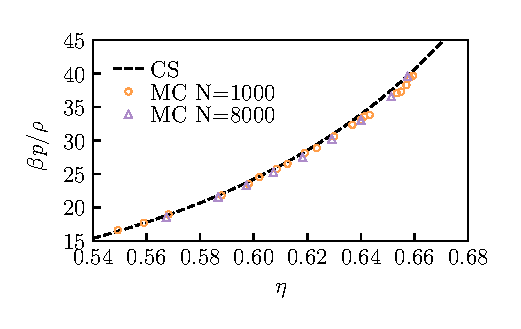
\includegraphics[width=0.9\linewidth,outer]{swap-cs-santos}
  \caption[Accuracy of Carnahan-Starling equation at high densities]{
    Accuracy of empirical Carnahan-Starling (CS) equation of state \eqref{eq:cs-mixtures} in the supercooled regime from comparison with novel Monte-Carlo (MC) simulations for a system with 23\% polydispersity.
    Simulation data reproduced from Ref.\ \cite{BerthierPRL2016}.
  }
  \label{fig:swap-eos}
\end{SCfigure}

Finally, we introduce the central approximation of chapters \ref{chapter:morphometric-framework}, \ref{chapter:morphometric-applications} and \ref{chapter:resummation} as a limit case of FMT.
The chemical potential of a new sphere $s$ can be determined as the free energy of a mixture where the limit where the new species is infinitely dilute, as in
\begin{equation}\label{eq:fmt-morphometric}
  \begin{split}
    \mu_s
    &=
    \lim_{\rho_s \to 0} \frac{\partial f^\mathrm{ex}}{\partial \rho_s}
    =
    \lim_{\rho_s \to 0}
    \sum_\alpha
    \frac{\partial n_\alpha}{\partial \rho_s}
    \frac{\partial f^\mathrm{ex}}{\partial n_\alpha},
    \\ &=
    \frac{\partial f^\mathrm{ex}}{\partial \xi_3} \frac{4 \pi R_s^3}{3}
    + \frac{\partial f^\mathrm{ex}}{\partial \xi_2} 4 \pi R_s^2
    + \frac{\partial f^\mathrm{ex}}{\partial \xi_1} R_s
    + \frac{\partial f^\mathrm{ex}}{\partial \xi_0}
  \end{split}
\end{equation}
using the explicit derivatives \eqref{eq:fmt-n-derivatives} in the second line.
Noting that the partial derivatives of $f^\mathrm{ex}$ are constants of the bulk liquid and the other contributions are normalisations of the intrinsic volumes (cf.\ table \ref{table:geometric-quantities}), the central conjecture of the morphometric approach is that this generalises to arbitrary shapes; that is, the chemical potential can be written \cite{KonigPRL2004,RothPRL2006}
\begin{equation}\label{eq:fmt-morphometric-2}
  \mu_s = p V_s + a_2 A_s + a_1 R_s + a_0
\end{equation}
with thermodynamic coefficients $\{p, a_2, a_1, a_0\}$ independent of the geometry.
We leave detailed discussion of this approximation until chapter \ref{chapter:morphometric-framework}, but for reference we will give the explicit coefficients for the already introduced FMT functionals below.

The thermodynamic coefficients in \eqref{eq:fmt-morphometric-2} can be determined for an FMT functional using the special case of spherical solutes \eqref{eq:fmt-morphometric}.
For the Rosenfeld functional \eqref{eq:rosenfeld-functional} we obtain the thermodynamic coefficients for the single-component hard sphere liquid
\begin{subequations}\label{eq:rosenfeld-coefficients}
  \begin{align}
    \beta a_0^\mathrm{RF}
    &=
    -\ln{(1- \eta)},
    \\
    \beta a_1^\mathrm{RF}
    &=
    \frac{6\eta}{\sigma (1 - \eta)},
    \\
    \beta a_2^\mathrm{RF}
    &=
    \frac{6\eta + 3\eta^2}{2\pi \sigma^2 (1 - \eta)^2},
    \\
    \frac{\beta p^\mathrm{RF}}{\rho}
    &=
    \frac{1 + \eta + \eta^2}{(1 - \eta)^3}.
    \label{eq:py-pressure}
 \end{align}
\end{subequations}
and for the CS functional \eqref{eq:santos-fmt} with \eqref{eq:cs-fmt} we find
\begin{subequations}\label{eq:wbii-coefficients}
  \begin{align}
    \beta a_0^\mathrm{WBII}
    &=
    - \ln{(1 - \eta)},
    \\
    \beta a_1^\mathrm{WBII}
    &=
    \frac{2}{\sigma} \left(
    \frac{5\eta + \eta^2}{1 - \eta}
    + 2 \ln{(1 - \eta)}
    \right),
    \\
    \beta a_2^\mathrm{WBII}
    &=
    \frac{1}{\pi \sigma^2} \left(
    \frac{\eta (2 + 3\eta - 2\eta^2)}{(1 - \eta)^2}
    - \ln{(1 - \eta)}
    \right),
    \\
    \frac{\beta p^\mathrm{WBII}}{\rho}
    &=
    \frac{1 + \eta + \eta^2 - \eta^3}{(1-\eta)^3},
 \end{align}
\end{subequations}
We label these as the White Bear II (WBII) coefficients because they were first derived from the WBII free energy functional%
\marginfootnote{These are not exactly as stated in Ref.\ \cite{Hansen-GoosJPCM2006} because we use a different definition of surface.
  The conversions between the different surfaces are stated in chapter \ref{chapter:morphometric-framework}: see the discussions around \eqref{eq:exclusion-transform}.}
\cite{Hansen-GoosJCP2006, Hansen-GoosJPCM2006} which is similar in form and construction to the CS functional described, although it is (marginally) less self-consistent.

%% \subsection{Superposition and convolution approximations}

%% \todo{Finish this section}
%% In the Kirkwood superposition approximation \cite{KirkwoodJCP1935} many-body correlations are expressed as pairwise products of the two-body correlation function, i.e.
%% \begin{equation}
%%   g^{(n)}(\vec{r}^n) =
%%   \prod_{i < j} g^{(2)}(\vec{r}_i, \vec{r}_j),
%% \end{equation}
%% which correctly satisfies the hard-core condition, but violates the sum rule
%% \begin{equation}
%%   \begin{aligned}
%%     \rho^{(n)}(\vec{r}^n) &=
%%     \frac{1}{\Xi} \sum_{N=n}^\infty \frac{z^N}{(N-n)!} \int e^{-\beta U_N} \, d\vec{r}^{(N-n)} \\
%%     &=
%%     \int d\vec{r}_n \left(
%%     \frac{1}{\Xi} \sum_{N=n}^\infty \frac{z^N}{(N+1 - (n+1))!} \int e^{-\beta U_N} \, d\vec{r}^{(N-(n+1))}
%%     \right) \\
%%     &=
%%     \int d\vec{r}_n \left(
%%     \frac{1}{\Xi} \sum_{N=n}^\infty \frac{z^N}{(N - (n+1))!} \int e^{-\beta U_N} \, d\vec{r}^{(N-(n+1))}
%%     \right) \\
%%     &=
%%     \frac{1}{N-n}
%%     \int \rho^{(n+1)}(\{\vec{r}^n, \vec{r}_{n+1}\}) d\vec{r}_{n+1},
%%   \end{aligned}
%% \end{equation}\todo{This is wrong.}
%% and the related convolution approximation \cite{JacksonRMP1962,IchimaruPRA1970,BarratMP1988}%
%% \todo{Check this expression is correct - it almost certainly is not.}
%% \begin{equation}
%%   S^{(n)}(\vec{k}^n) =
%%   (1 + \tilde{c}^{(n)}(\vec{k}^n))
%%   \prod_{i < j} S^{(2)}(\vec{k}_i, \vec{k}_j)
%% \end{equation}
%% satisfies the sum rule but fails to satisfy the hard-core condition.

%% In equilibrium
%% \begin{equation}
%%   c^{(n)}(\vec{r}^n) =
%%   \left.
%%   \frac{\delta^n \beta F_{ex}}{\delta \rho(\vec{r}_1)\delta \rho(\vec{r}_2) \cdots \delta \rho(\vec{r}_n)}
%%   \right|_{\rho(\vec{r})=\rho}
%% \end{equation}
